\documentclass{article}
\usepackage[utf8]{inputenc}
\usepackage{graphicx}
\usepackage{parskip}
\usepackage{xcolor}
\usepackage{textcomp}
\usepackage{hyperref}
\hypersetup{
    colorlinks=true,
    linkcolor=blue,
    filecolor=magenta,      
    urlcolor=cyan,
}
\usepackage{listings}
\lstset{language=C,
                backgroundcolor = \color{lightgray},
                showstringspaces = false,
                basicstyle=\ttfamily,
                keywordstyle=\color{blue}\ttfamily,
                stringstyle=\color{red}\ttfamily,
                commentstyle=\color{green}\ttfamily,
                morecomment=[l][\color{magenta}]{\#}
}

\title{The Vending Machine - Code Documentation}
\author{By \\ Umang Deshpande and Akshay Hegde}
\date{June 2017}

\begin{document}
\maketitle

\section{Program Code}
\qquad The git repository for the complete code can be found \href{https://github.com/eYSIP-2017/eYSIP-2017_Game_Development-TI-RTOS/tree/master/VendingMachine_Final}{here}. It contains the complete project folder used in CCS. 
\begin{itemize}
  \item The console support libraries are present in the \href{https://github.com/eYSIP-2017/eYSIP-2017_Game_Development-TI-RTOS/tree/master/VendingMachine_Final/Console}{Console} folder. 
  \item The font and graphic libraries are present in the \href{https://github.com/eYSIP-2017/eYSIP-2017_Game_Development-TI-RTOS/tree/master/VendingMachine_Final/Images}{Images} folder.
  \item VM\_RTOS.c is the main file. This contains the Statechart and RTOS implementation of the vending machine abstraction.
\end{itemize}

\section{Main Code}
\qquad Firstly, following headers are included:
  \begin{lstlisting}[basicstyle = \small, language = C]
/* XDC module Headers */
#include <xdc/std.h>
#include <xdc/runtime/System.h>


//needed for any Log_info() call
#include <xdc/runtime/Log.h>
//header file for statically defined objects/handles
#include <xdc/cfg/global.h>
//needed for any Log_info() call
#include <xdc/runtime/Log.h>


/* BIOS module Headers */
#include <ti/sysbios/BIOS.h>
#include <ti/sysbios/knl/Clock.h>
#include <ti/sysbios/knl/Task.h>
#include <ti/sysbios/knl/Semaphore.h>


/* Standard CHeader files*/
#include <stdint.h>
#include <stdbool.h>
#include <string.h>
#include <time.h>

/* Custom Game Console Header */
#include "Console/console.h"
#include "Console/glcd.h"

/* Timer and GPIO function Headers */
#include "driverlib/timer.h"
#include "inc/hw_memmap.h"

/*For ROM Functions*/
#define TARGET_IS_BLIZZARD_RB1
#include "driverlib/rom.h"

/*
 * This Header files for all custom imagery 
   including smiley, soda can, coin graphic.
 */
#include "Images/images.h"
  \end{lstlisting}
\begin{itemize}
  \item XDC Headers handle XDCTools as part of RTOS, which aid in debugging.
  \item BIOS module headers allow use of Tasks and Semaphore definitions.
  \item \texttt{stdint.h} Headers allow use of \texttt{uint32} variables, stdbool allows use of \texttt{stdbool.h} variables, \texttt{string.h} allows manipulation of string in string variables, \texttt{time} allows for use of the time functions for block randomization.
  \item The Console headers provide developer level functions to the console, so that initialization can be performed using a single function \texttt{\_init\_()}. And GLCD functions for direct display of fonts and graphic are obtained from \texttt{glcd.h} header.
  \item For the timer and timer interrupt functions used in Timer ISR(Task Scheduler), \texttt{timer.h} and \texttt{hw\_memmap.h} are used.
  \item \texttt{rom.h} Allows the use of ROM functions for the given board.
  \item \texttt{images.h} Contains various different images in the form of hex arrays to be displayed on screen.
\end{itemize}
\newpage
\qquad Following this, define all global variables are defined as follows:
  \begin{lstlisting}[basicstyle = \small, language = C]
/*
 * Global Variables
 */

uint32_t latency, pinName, baseName, flag;
volatile uint32_t tickCount=0;
signed int sum;
char digits[4] = "00c";
char text[];
unsigned char p, ch, reg_n, diet_n, holder, character;
unsigned char temp[8];
  \end{lstlisting}
\begin{itemize}
  \item \texttt{pinName},\texttt{baseName} and \texttt{flag} are used for Switch selection. \texttt{baseName} is the port to which the switch belongs to. \texttt{pinName} is the actual pin to which the switch is connected.
  \item \texttt{tickCount} is used for Task Scheduling in \texttt{Timer\_ISR}.
  \item \texttt{sum} holds the total money entered into the vending machine
  \item \texttt{digits[4]} is used to hold the sum entered in string format to display total money entered on GLCD.
  \item \texttt{text[]},\texttt{ch}, \texttt{temp[8]} and \texttt{character} hold text to be displayed on GLCD.
  \item \texttt{reg\_n} and \texttt{diet\_n} holds total number of regular and diet sodas requested by the user.
\end{itemize}
\qquad All the different states for the various state machines used are enlisted as follows:
  \begin{lstlisting}[basicstyle = \small, language = C]
/*
 * Enumeration of States for State Machine
 */
enum vm_modes{

    // States for Vending Machine

    INITM,
    COIN,
    SELECT,
    DELIVERY
};
// Initialization
enum vm_modes vm_mode = INITM;
  \end{lstlisting}
  \texttt{vm\_mode} enumerated variable is thus initially in \texttt{INITM} state.
    \begin{lstlisting}[basicstyle = \small, language = C]
  enum inputs{

    // Different input transitions enumeration

    INITI,
    DIME,
    NICKEL,
    QUARTER,
    NONEI
};
// Initialization
enum inputs input = INITI;
  \end{lstlisting}
    \texttt{input} enumerated variable is thus initially in \texttt{INITI} state.
    \begin{lstlisting}[basicstyle = \small, language = C]

enum outputs{

    //Output internal states enumeration

    INITO,
    REGULAR,
    DIET,
    CHANGE,
    NONEO
};

//Initialization
enum outputs output = INITO;
  \end{lstlisting}
    \texttt{output} enumerated variable is thus initially in \texttt{INITO} state. \\
\qquad Following this, various functions are defined as follows:
\begin{itemize}
  \item \texttt{coinScreenInput()}. This function detects which coin has been entered through switch press detection. Handles inputs in COIN state. Calculate sum based on input transition. Also transition to next Vending Machine state. The state machine(internal is as in Fig c.
      \begin{lstlisting}[basicstyle = \small, language = C]
void coinScreenInput()
{
    // Update the total Sum to be displayed
    digits[1] = (sum%10) + '0';
    digits[0] = (sum/10) + '0';
    if(detectKeyPress(0) == 1)
    {
        // UP Switch Pressed 
        // -> Entered Dime
        input = DIME;
        sum += 5;
        micros(50);
        glcd_clearDisplay();
    }
    else if(detectKeyPress(2) == 1)
    {
        // DOWN Switch Pressed 
        // -> Entered Nickel
        input = NICKEL;
        sum += 10;
        micros(50);
        glcd_clearDisplay();
    }
    else if(detectKeyPress(4) == 1)
    {
        // HAT Switch Pressed(On Thumbstick) 
        // -> Entered Quarter
        input = QUARTER;
        sum += 25;
        micros(50);
        glcd_clearDisplay();
    }
    else if(detectKeyPress(1) == 1)
    {
        // RIGHT Switch Pressed 
        // -> Go to Selection Screen
        vm_mode = SELECT;
    }
}
  \end{lstlisting}
  \item \texttt{coinScreenDisplay()}.This function displays GUI to user in the COIN state. Handles GLCD. Changes graphic and text displayed based on input transition. The state machine(internal) is as in Fig a.
      \begin{lstlisting}[basicstyle = \small, language = C]
void coinScreenDisplay()
{
    switch(input){
    case INITI:
        // Display Home Screen with COIN graphic 
        // and text. Switch to No Coin Inserted State.
        glcd_write(coin);
        displayText("  5c>Press UP    10c>Press DOWN
        25c>Press HAT  Next>Press RIGHT", 4);
        input = NONEI;
        break;
    case DIME:
        // DIME input detected. Total Money 
        // Entered Displayed. Further provision 
        // to enter more coins.
        displayText(digits, 0);
        displayText("Entered
        5c>Press UP     10c>Press DOWN  25c>Press HAT
        Next>Press RIGHT", 1);
        break;
    case NICKEL:
        // NICKEL input detected. Total Money 
        // Entered Displayed. Further provision 
        // to enter more coins.
        displayText(digits, 0);
        displayText("Entered 
        5c>Press UP     10c>Press DOWN  25c>Press HAT
        Next>Press RIGHT", 1);
        break;
    case QUARTER:
        // QUARTER input detected. Total Money 
        // Entered Displayed. Further provision to enter 
        // more coins.
        displayText(digits, 0);
        displayText("Entered
        5c>Press UP     10c>Press DOWN  25c>Press HAT
        Next>Press RIGHT", 1);
        break;
    case NONEI:
        // No Input detected.
        break;
    }
}
  \end{lstlisting}
  \item \texttt{selectScreenInput()}. This function selects soda based on switch press. Can select multiple soda at once. Dispensed based on money entered. Handles Input in SELECT state. Also transition to next Vending Machine state. The state machine(internal) is as in Fig c.
      \begin{lstlisting}[basicstyle = \small, language = C]
void selectScreenInput()
{
    if(detectKeyPress(3) == 1)
    {
        // LEFT Switch Pressed 
        // -> Selected Regular Soda, cost 35c.
        sum -= 35;
        reg_n++;
        output = REGULAR;
        glcd_clearDisplay();
    }
    else if(detectKeyPress(1) == 1)
    {
        // RIGHT Switch Pressed 
        // -> Selected Diet Soda, cost 35c.
        sum -= 35;
        output = DIET;
        diet_n++;
        glcd_clearDisplay();
    }
    else if(detectKeyPress(0) == 1)
    {
        // UP Switch Pressed 
        // -> Abort Transaction. No Soda Selected.
        output = CHANGE;
        glcd_clearDisplay();
    }
    else if(detectKeyPress(2) == 1)
    {
        // DOWN Switch Pressed 
        // -> Continue to Delivery State.
        vm_mode = DELIVERY;
    }
}
  \end{lstlisting}
  \item \texttt{selectScreenDisplay()}. This function displays GUI in SELECT state. Change screens based on Soda Selection. The state machine(internal) is as in Fig a.
      \begin{lstlisting}[basicstyle = \small, language = C]
void selectScreenDisplay()
{
    switch(output)
    {
    case INITO:
        // Display Initial Selection Screen, with 
        // Soda Can Graphic.
        glcd_clearDisplay();
        display40x32(0, 3, soda_can);
        displayText("Reg>Press LEFT  
        Diet>Press RIGHTCancel>Press UP", 5);
        output = NONEO;
        break;
    case REGULAR:
        // Regular Soda Selected Screen.
        displayText("Selected Regular                
        Reg>Press LEFT  Diet>Press RIGHTContinue>Press
        DOWN", 2);
        break;
    case DIET:
        // Diet Soda Selected Screen.
        displayText("Selected Diet                   
        Reg>Press LEFT  Diet>Press RIGHTContinue>Press
        DOWN", 2);
        break;
    case CHANGE:
        // Abort transaction, no soda selected Screen.
        displayText("Abort Transaction                
        Continue>Press  DOWN", 2);
        break;
    case NONEO:
        // Undefined state.
        break;
    }
}
  \end{lstlisting}
  \item \texttt{deliveryOutput()}. This function displays GUI in DELIVERY state. Additionally, also in charge of LED blink delivery indication. Certain screens are displayed based on dispensed soda and change, in addition to LED blinks. The state machine(internal) is as in Fig b.
      \begin{lstlisting}[basicstyle = \small, language = C]
void deliveryOutput()
{
    switch(output){
    case REGULAR:
        // Regular Soda Output
        if(sum >= 0)
        {
            // Provided enough coins entered, 
            // Display Soda Delivery LED blink 
            // and GLCD Screen with Smiley Graphic.
            glcd_clearDisplay();
            display40x32(1, 3, smiley);
            displayText("  Please Enjoy     
            Your Drink!", 5);
            while(reg_n > 0)
            {
                // Blink LED as many times as 
                // number of Regular Sodas Selected.
                ledON(1);
                millis(1000);
                ledOFF(1);
                millis(1000);
                reg_n--;
            }
        }
        else
        {
            // If coins are not sufficient for 
            // the transaction, display refusal screen.
            sum =+ ((diet_n+reg_n)*35);
            glcd_clearDisplay();
            displayText(" Sorry, unable to dispense.
            Insufficient Cash", 2);
        }
        // Switch to CHANGE output state.
        output = CHANGE;
        break;
    case DIET:
        // Diet Soda Output
        if(sum >= 0)
        {
            // Provided enough coins entered, 
            // Display Soda Delivery LED blink 
            // and GLCD Screen with Smiley Graphic.
            glcd_clearDisplay();
            display40x32(1, 3, smiley);
            displayText("  Please Enjoy     
            Your Drink!", 5);
            while(diet_n > 0)
            {
                // Blink LED as many times as 
                // number of diet sodas selected.
                ledON(2);
                millis(1000);
                ledOFF(2);
                millis(1000);
                diet_n--;
            }
        }
        else
        {
            // If coins are not sufficient for the 
            // transaction, display refusal screen.
            sum += ((diet_n+reg_n)*35);
            glcd_clearDisplay();
            displayText(" Sorry, unable  to dispense. 
            In-sufficient Cash", 2);
            millis(2000);
        }
        output = CHANGE;
        break;
    case CHANGE:
        // Deliver change output screen display
        glcd_clearDisplay();
        glcd_write(coin);
        displayText("    Collect         Change", 6);
        millis(2000); 
        // Continue to blink LED until all change 
        // is returned. Change is given as 5c each 
        //per LED blink.
        while(sum > 0)
        {
            ledON(3);
            millis(500);
            ledOFF(3);
            millis(500);
            sum -= 5;
        }
        // Display Thank you screen.
        glcd_clearDisplay();
        displayText(" Thank you for  using SodVen
         Vending Machine!", 2);
        millis(2000);
        glcd_clearDisplay();
        // Switch Back to Initial State.
        vm_mode = INITM;
        break;
    }
}
  \end{lstlisting}
    \item \texttt{updateOutput()}. This implements the output vending machine statechart as depicted in Fig a and Fig b. Various internal state machines are implemented using each function. Switches between various screens in different Vending Machine states. Is implemented as a task in RTOS, initialized with OutputSem Semaphore.
      \begin{lstlisting}[basicstyle = \small, language = C]
void updateOutput(void)
{
    while(1)
    {
        Semaphore_pend(OutputSem, BIOS_WAIT_FOREVER);

        // Output Control State Machine.
        switch(vm_mode){
        case INITM:
            // Resets various variables.
            sum = 0;
            reg_n = 0;
            diet_n = 0;
            vm_mode = COIN;
            input = INITI;
            output = INITO;
        case COIN:
            coinScreenDisplay();
            break;
        case SELECT:
            selectScreenDisplay();
            break;
        case DELIVERY:
            deliveryOutput();
            break;
        }
    }
}
  \end{lstlisting}
 \item Vending Machine Statechart(Output).
\begin{center}
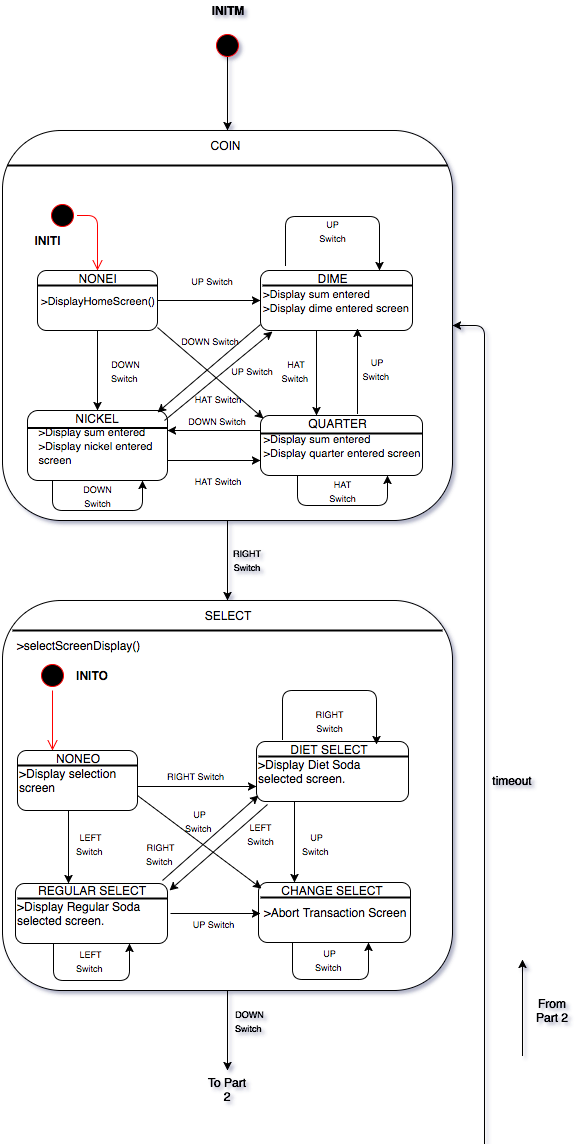
\includegraphics[width=10cm, height=18cm]{vendingMachineOutput1}
\\ {\small Fig a: Vending Machine Output Statechart Part 1}
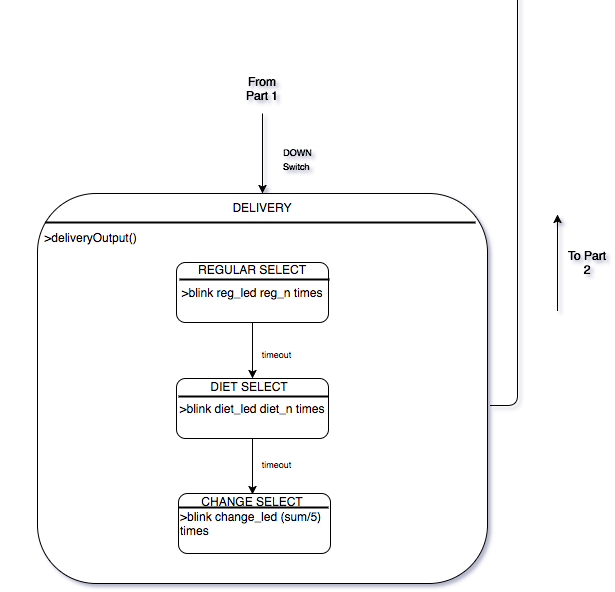
\includegraphics[width=10cm, height=8cm]{VendingMachineOutput2}
\\ {\small Fig b: Vending Machine Output Statechart Part 2}
\end{center}
 \item \texttt{readInput()}. This function implements the Vending Machine Statechart depicted in Fig c and Fig d(Following code snippet). Internal state machines are implemented within each function as described above.Is implemented as a task in RTOS, initialized with SwitchSem Semaphore.
 \begin{lstlisting}[basicstyle = \small, language = C]
void readInput(void)
{
    while(1)
    {
        Semaphore_pend(SwitchSem, BIOS_WAIT_FOREVER);
        // Input Control State Machine.
        switch(vm_mode){
        case INITM:
            break;
        case COIN:
            coinScreenInput();
            break;
        case SELECT:
            selectScreenInput();
            break;
        case DELIVERY:
            // No user input in delivery state
            break;
        }
    }
}
  \end{lstlisting}
\item Vending Machine Statechart(Input).
\begin{center}
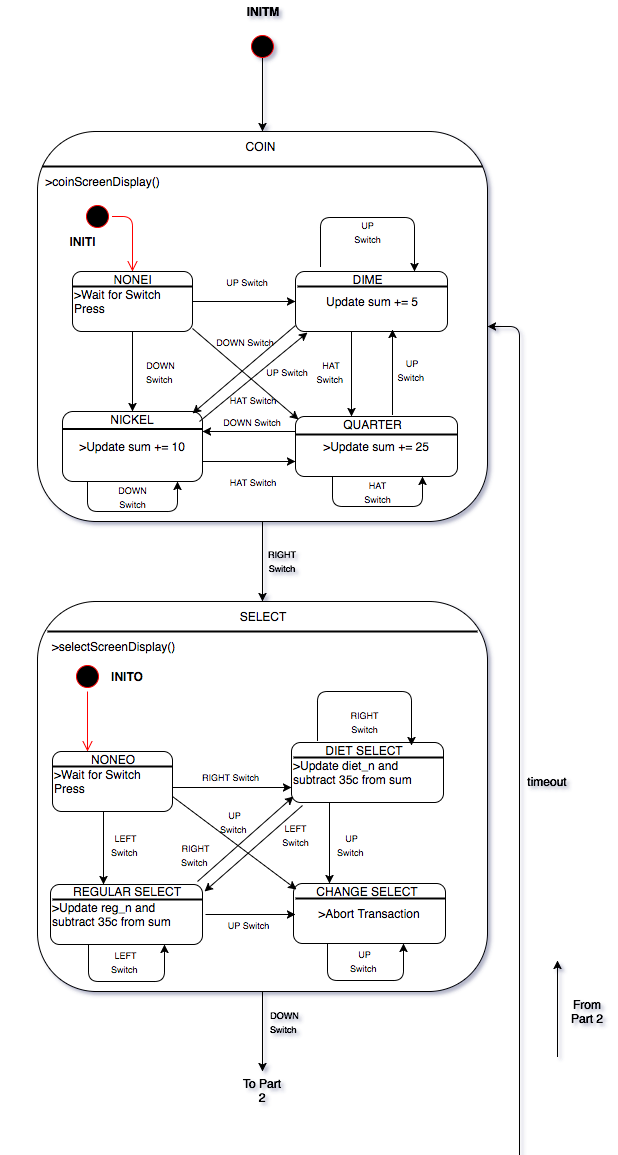
\includegraphics[width=10cm, height=18cm]{VendingMachineInput1}
\\ {\small Fig c: Vending Machine Input Statechart Part 1}
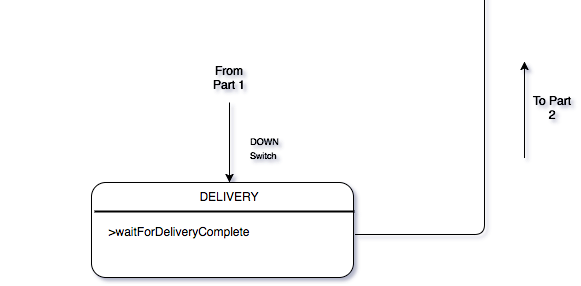
\includegraphics[width=10cm, height=4cm]{vendingMachineInput2}
\\ {\small Fig d: Vending Machine Input Statechart Part 2}
\end{center}
\end{itemize}
\qquad \texttt{main()} function serves to initialize and start the BIOS. The BIOS handles program execution. Now, the \texttt{main()} function is defined as follows:
      \begin{lstlisting}[basicstyle = \small, language = C]
int main(void)
{
    /* Set display refresh latency */
    latency = 40;
    
    /* Initialize all peripherals, GPIOs, 
    Interrupts and GLCD. */
    _init_();
    glcd_init();
    glcd_clearDisplay();
    
    /* Turn off all LEDs*/
    ledOFF(1);
    ledOFF(2);
    ledOFF(3);
    ledOFF(4);
    
    /* Start BIOS */
    BIOS_start();

    return (0);
}
  \end{lstlisting}
\qquad Finally, the \texttt{Timer\_ISR()} is defined, which implements the task scheduling as shown: \\ \\
      \begin{lstlisting}[basicstyle = \small, language = C]
void Timer_ISR(void)
{
    // Clear Timer Interrput
    ROM_TimerIntClear(TIMER2_BASE, TIMER_TIMA_TIMEOUT);
    // Increment tickCount used for Scheduling
    tickCount++;
    // Task Scheduler
    switch(tickCount){
    case 15:
        // Post Switch Semaphore
        Semaphore_post(SwitchSem);
        break;
    case 30:
        // Post Output Semaphore
        Semaphore_post(OutputSem);
        // Reset tickCount
        tickCount = 0;
        break;
    }
}
  \end{lstlisting}
This is the complete code for the Vending Machine Controller, with a state machine implementation.
\end{document}
